In this section we will present some preliminary results of our VM.
First, we present scalability results in order to show that LM programs take advantage of the advantages of multicore architectures.
Next, we present some absolute execution times and a comparison with similar programs in other programming languages.
We want to present evidence that LM is a viable and competitive language.

For our experimental setup, we used a machine 
with two 16 (32) Core AMD Opteron
(tm) Processor 6274 $@$ 2.2 GHz with 32 GBytes of RAM memory and running the Linux
kernel 3.8.3-1.fc17.x86\_64.
     We compiled our VM using GCC 4.7.2 (g++) with the flags \texttt{-O3 -std=c+0x -march=x86-64}.
     We run all experiments 3 times with the same configuration and then we averaged the execution time.
     
\subsection{Scalability Results}

For this section, we run each program using 1, 2, 4, 6, 8, 10, 12, 14 and 16 threads and compared the runtime against the execution of the sequential version of the VM. We used the following programs:

\newcommand{\figsize}[0]{6.5cm}
\captionsetup[sub]{              % The subcaption settings
       font=scriptsize}

\begin{description}
   \item[Greedy Graph Coloring (GGC)] this program colors nodes in a graph so that no two adjacent nodes have the same color. We start with a small number of colors and then we expand the number of colors when we cannot color the graph.
   \item[PageRank] implements an asynchronous PageRank algorithm without synchronization between iterations. Every time a node sends a new rank to its neighbors and the change was significant, the neighbors are scheduled to recompute their ranks.
   \item[N queens] implements the N Queens problem, as explained before, for a 13x13 board.
   \item[Belief propagation] machine learning algorithm to denoise a 400x400 image.
\end{description}

Figure~\ref{exp:graph_coloring} presents the speedup results for the GGC program using 2 different datasets. In Fig.~\ref{exp:graph_coloring}~(a) we show the speedup for a graph of 12,000 webpages\footnote{The search engine graph was retrieved from \url{http://www.cs.toronto.edu/~tsap/experiments/download/download.html}}. Since this dataset follows the power law, that is, there is a small number of pages with a lots of links (1\% of the nodes have 75\% of the edges), the speedup is slightly worse than the benchmark shown in Fig.~\ref{exp:graph_coloring}~(b), where we use a random dataset of 2,000 nodes and an uniform distribution of edges.

\begin{figure*}[h]
   \centering
   \begin{subfigure}[b]{0.40\textwidth}
      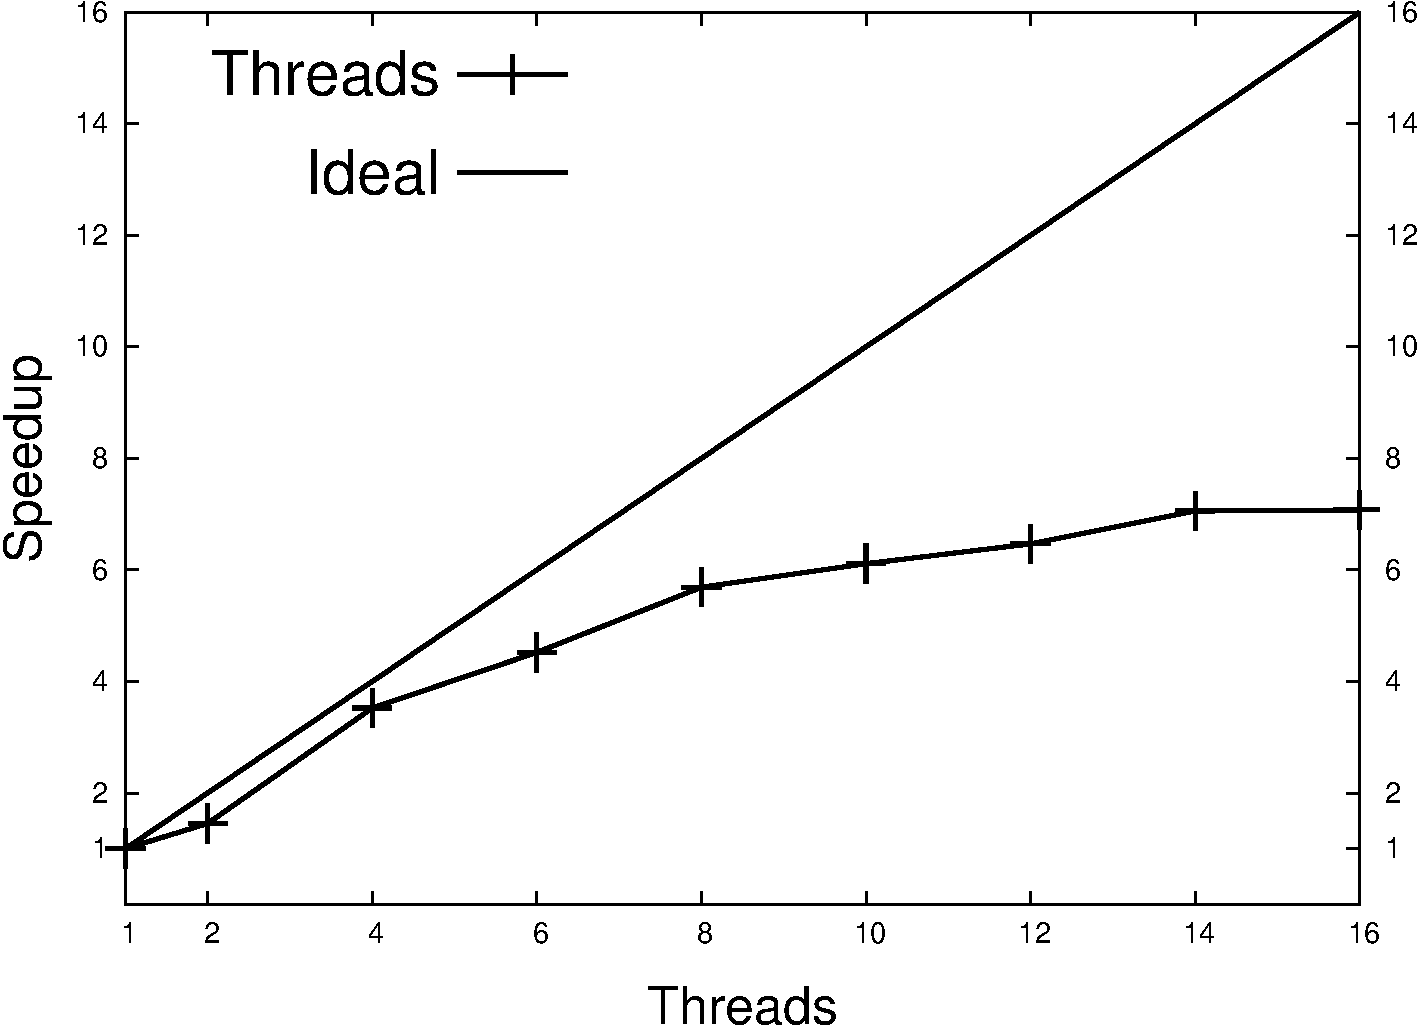
\includegraphics[width=\textwidth]{speedup_greedy-graph-coloring-search_engines.pdf}
      \caption{Using a graph of web pages collected from a search engine (around 12,000 nodes and 292,000 edges).}
   \end{subfigure}
   \begin{subfigure}[b]{0.40\textwidth}
      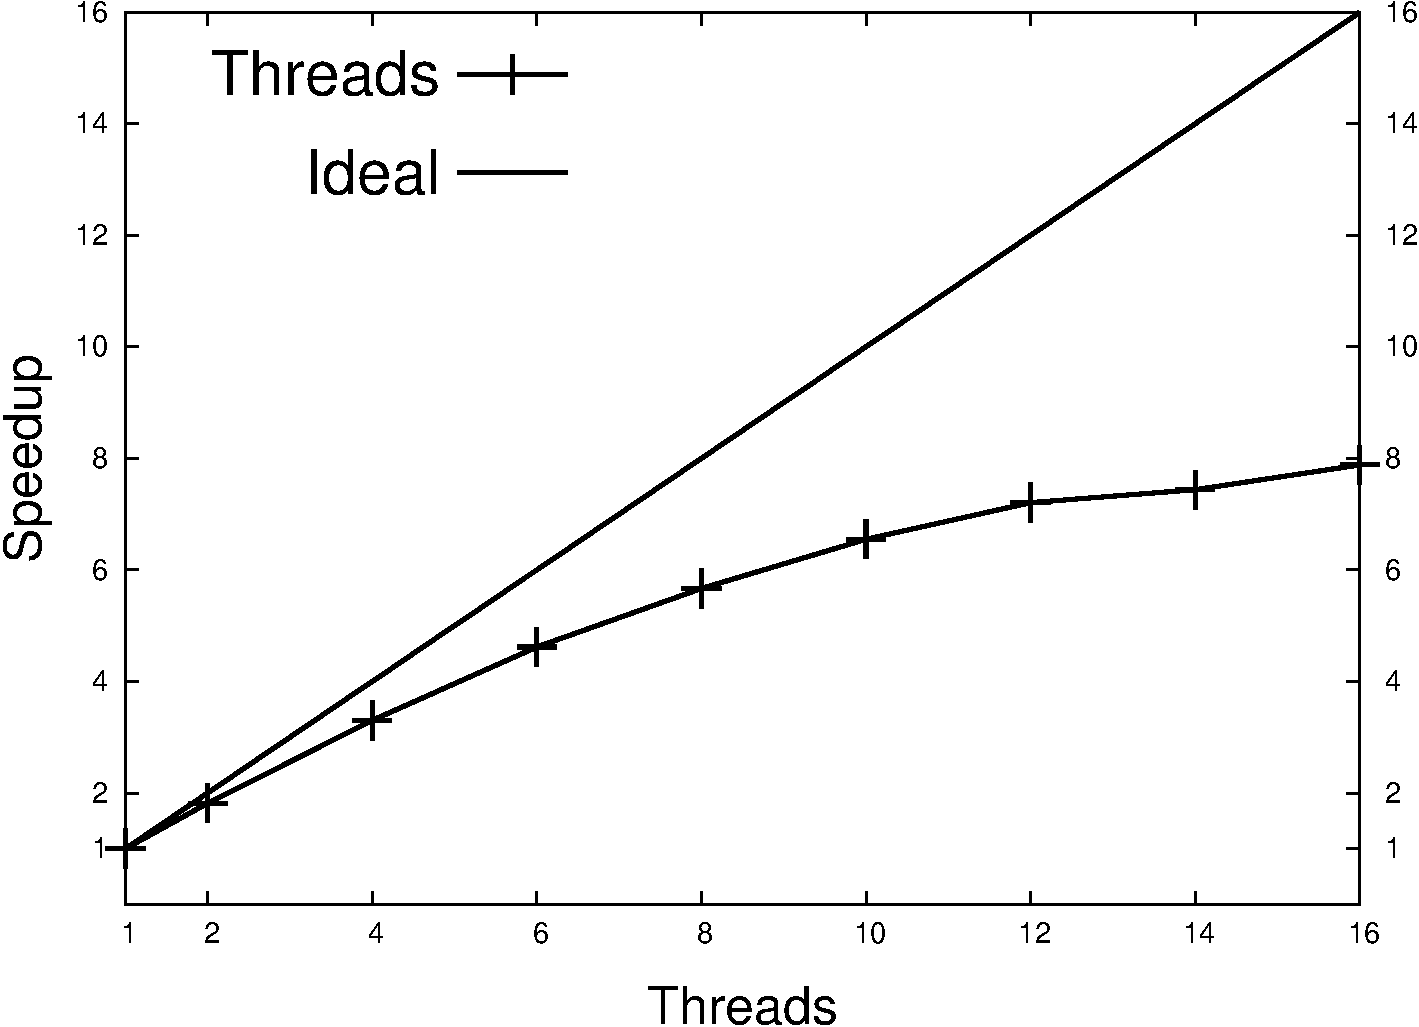
\includegraphics[width=\textwidth]{speedup_greedy-graph-coloring-2000.pdf}
      \caption{Using a random graph with 2,000 nodes and 600,000 edges.\newline}
   \end{subfigure}
   \caption{Experimental results for the greedy GGC algorithm.}
   \label{exp:graph_coloring}
\end{figure*}

The PageRank results are shown in Fig.~\ref{exp:pagerank}. We used the same search engine dataset as before and a new random dataset with 5000 nodes and 500,000 edges. Although the search engine graph (Fig.~\ref{exp:pagerank}~(a)) has half the edges (around 250,000), it scales better than the random graph (Fig.~\ref{exp:pagerank}~(b)), meaning that the PageRank program depends on the number of nodes to be more scalable.

\begin{figure*}[h]
   \centering
   \begin{subfigure}[b]{0.40\textwidth}
      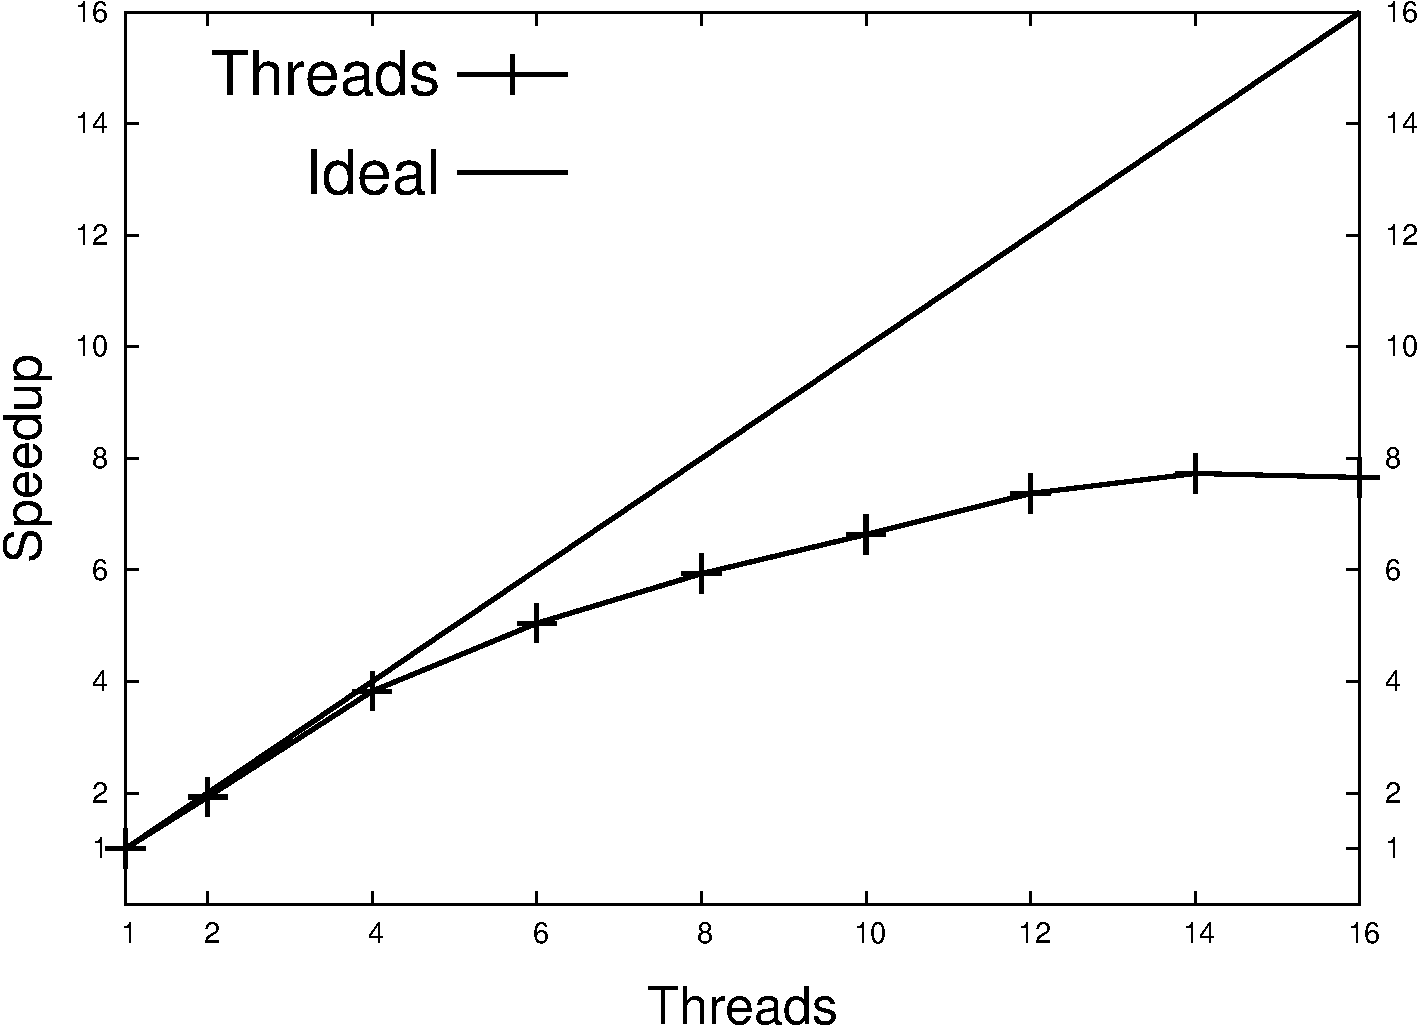
\includegraphics[width=\textwidth]{speedup_pagerank-search_engines.pdf}
      \caption{Using a graph of web pages collected from a search engine (around 12,000 nodes and 292,000 edges)}
   \end{subfigure}
   \begin{subfigure}[b]{0.40\textwidth}
      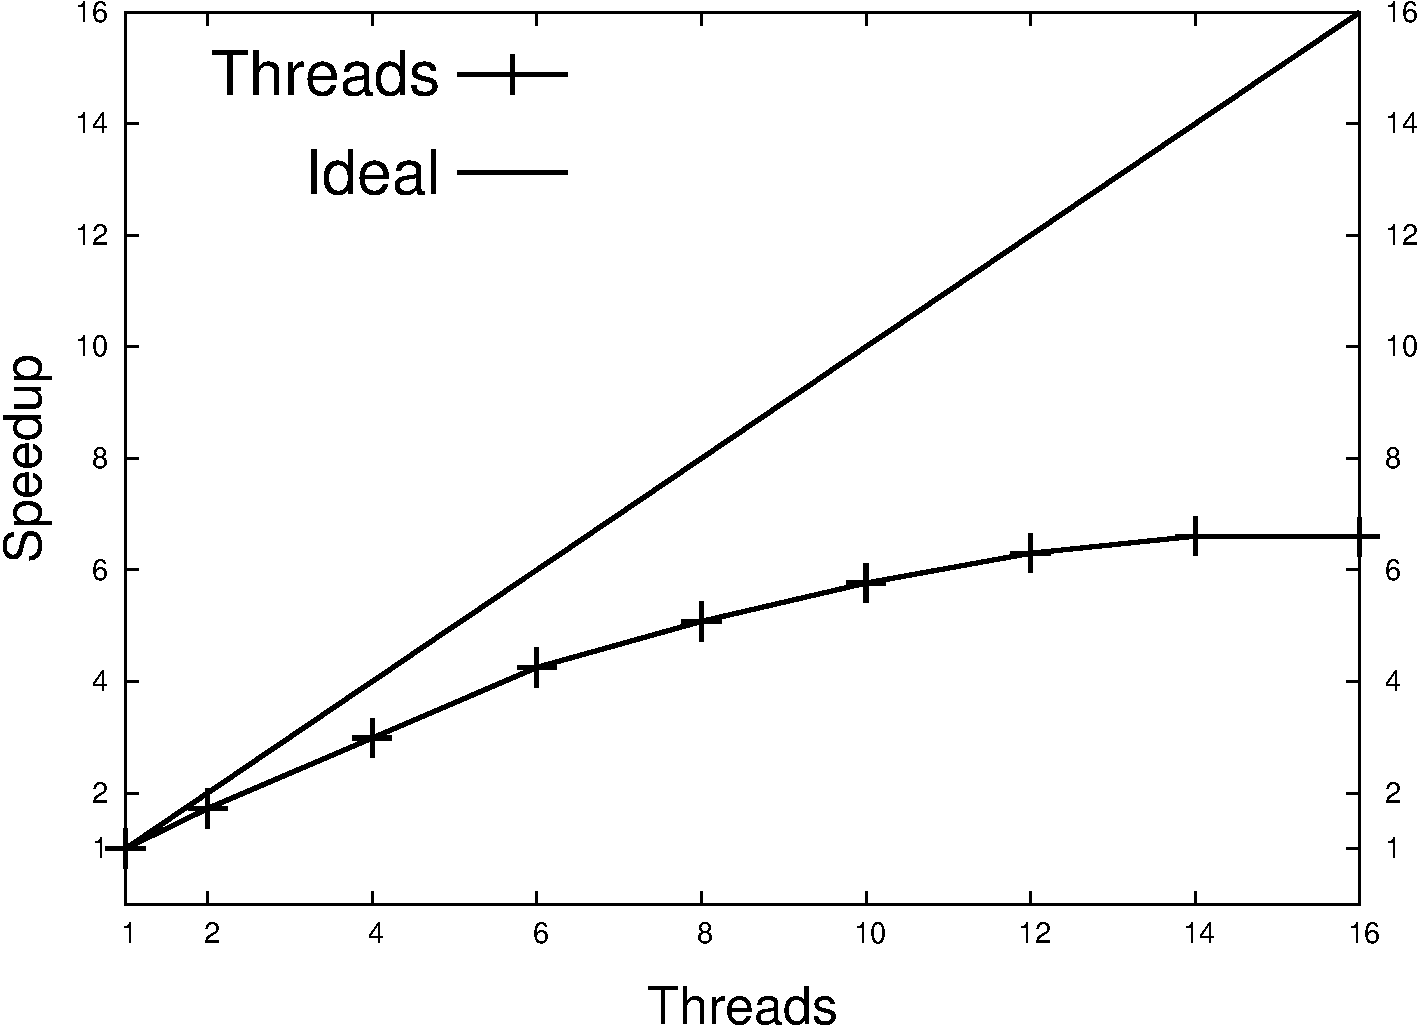
\includegraphics[width=\textwidth]{speedup_pagerank-5000.pdf}
      \caption{Using a random graph with 5,000 nodes and 500,000 edges.\newline}
   \end{subfigure}
   \caption{Experimental results for the asynchronous PageRank algorithm.}
   \label{exp:pagerank}
\end{figure*}

\begin{figure*}[h]
   \centering
   \begin{subfigure}[b]{0.40\textwidth}
      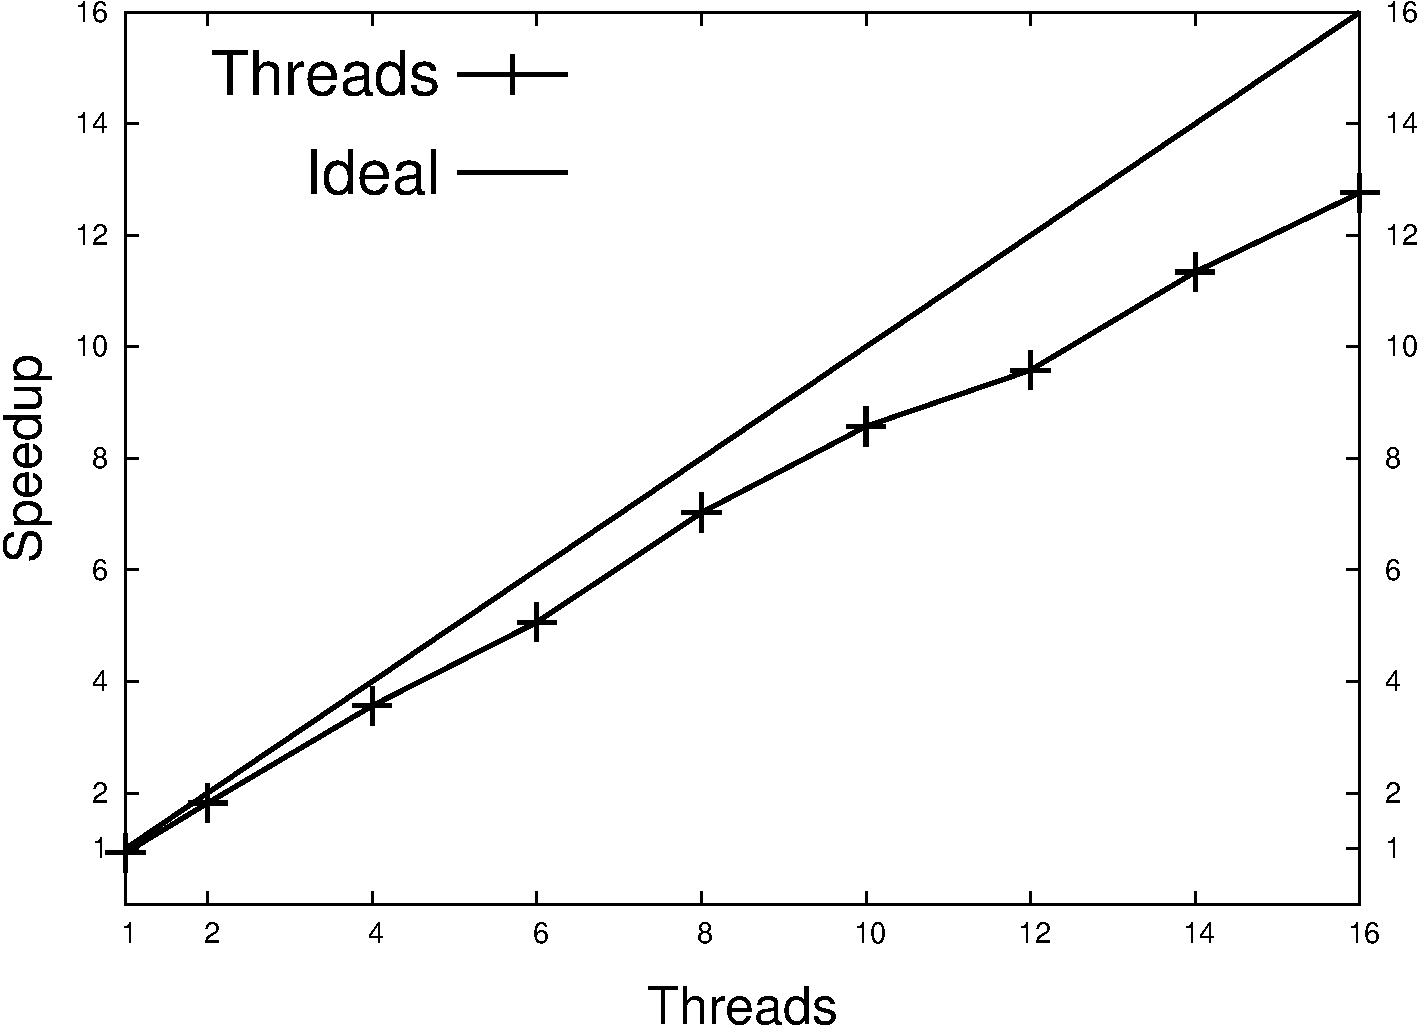
\includegraphics[width=\textwidth]{speedup_8queens-13.pdf}
      \caption{Experimental results for the N queens program (13x13~board).}
      \label{exp:8queens}
   \end{subfigure}
   \begin{subfigure}[b]{0.40\textwidth}
      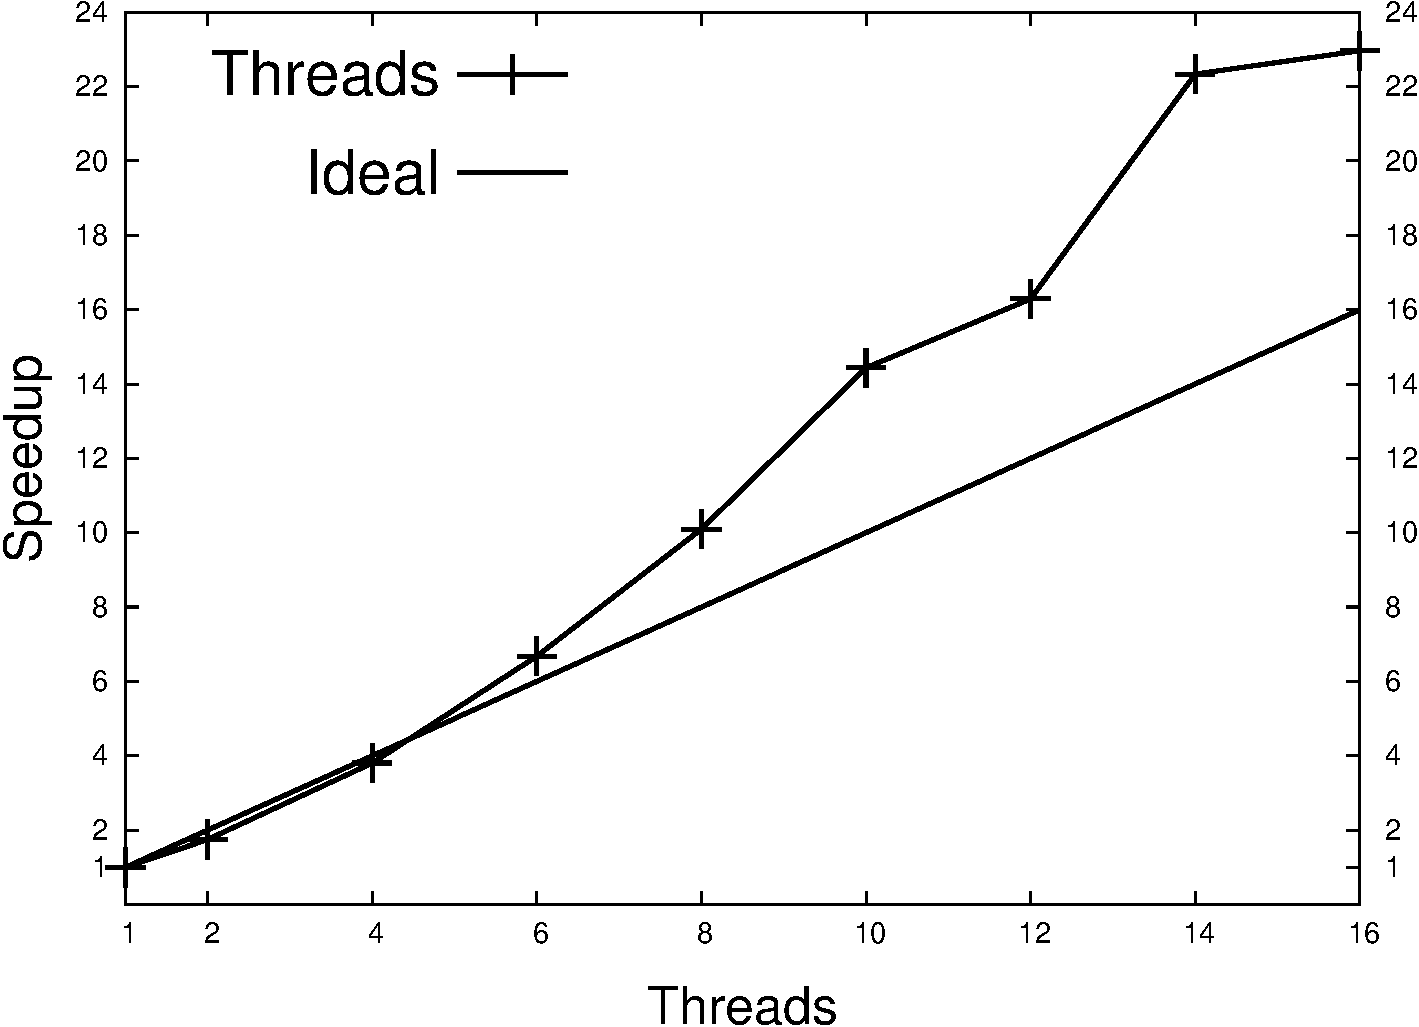
\includegraphics[width=\textwidth]{speedup_bp-400.pdf}
      \caption{Experimental results for the Belief Propagation program (400x400~image).}
      \label{exp:bp}
   \end{subfigure}
\end{figure*}

The results for the N queens program are shown in Fig.~\ref{exp:8queens}. The program is not regular since computation starts at the top of the grid and then rolls down, until only the last row is doing computation. Because the number of valid states for the nodes in the upper rows is much less than the nodes in the lower rows, this may create potential load balancing problems. The results show that our system is able to scale well due to work stealing.

Finally, we have the Belief Propagation~(BP) program in Fig.~\ref{exp:bp}. BP is very regular and asynchronous program and it benefits
from having multiple threads executing since the belief values of each node will converge faster. The super-linear results prove this
assertion.

\subsection{Absolute Execution Time}

As we have seen, our VM scales reasonably well, but how does it fair in terms of absolute execution time? We now compare the execution
time using one thread against other competing systems.

In Table~\ref{comp:nqueens} we compare the LM's N-Queens version against 3 other versions: a straightforward sequential program implemented
in C using backtracking; a sequential Python\cite{vanRossum:1995:PRM} implementation; and a Prolog implementation executed in
YAP Prolog~\cite{DBLP:journals/corr/abs-1102-3896}, an efficient implementation of Prolog. Numbers less than 1 mean that LM
is faster and larger than 1 mean that LM is slower. We see that LM easily beats Python, but is 5 to 10 times slower than YAP
and around 15 times slower than C.
However, note that if we use at least 16 threads in LM, we can beat the sequential implementation written in C.

\begin{figure}[h]
   \centering
    \begin{tabular}{ | l | l | l | l |}
    \hline
    
    Problem size & C & Python & YAP Prolog \\ \hline\hline
    10 & 16.92 & \textbf{0,62} & 5,42 \\
    11 & 21.59 & \textbf{0.64} & 6.47 \\
    12 & 10.32 & \textbf{0.73} & 7.61 \\
    13 & 14.35 & \textbf{0.88} & 10.38 \\
    \hline
    \end{tabular}
    \caption{Comparing absolute execution time for the N-Queens problem (System Time / LM Time).}
    \label{comp:nqueens}
\end{figure}

\begin{figure}[h]
   \centering
    \begin{tabular}{ | l | l | l | l |}
    \hline
    
    Problem size & C & Python & GraphLab \\ \hline\hline
    10 & \textbf{0.67} & \textbf{0,62} & \textbf{1.00} \\
    50 & \textit{1.77} & \textbf{0.64} & \textit{1.73} \\
    200 & \textit{1.99} & \textbf{0.73} & \textit{1.79} \\
    400 & \textit{2.00} & \textbf{0.88} & \textit{1.80} \\
    \hline
    \end{tabular}
    \caption{Comparing absolute execution time for the Belief Propagation program (System Time / LM Time).}
    \label{comp:bp}
\end{figure}